\chapter{Methodology and Implementation}\label{chap:meth_and_impl}

	\paragraph{ } Here in this chapter we will discuss the methods applied to extract an explicit model from an \ac{epr} problem specification. And how they are implemented using E's data structures and configurations.

	\paragraph{    In order to achieve our goal,} we had to transform the problems' clauses, which are the axioms of the specification and the negated conjectures(if found), to clauses in range restricted form through a simplified form of range restricted transformations. The original range restricted transformations and there simplified version will be discussed in section \ref{sec:c3s1}.  

	\section{Transformations}\label{sec:c3s1}
The methods applied in the project to extract the models follows the transformations discussed in \cite{BMUG06}. A brief on the original transformations will be given in \ref{sub:c3s1s1}.


Moreover, as mentioned before that this project is concerned with a sub-class of \ac{fol} which is \ac{epr} some simplifications to the transformations were made as the removed steps will have no meaning in the context of \ac{epr} problems. Those simplifications will be discussed in \ref{sub:c3s1s2}.

	\subsection{Original transformations}\label{sub:c3s1s1}
	\paragraph{The original procedures} discussed in \cite{BMUG06} generally work for all sub-classes of \ac{fol}. Those procedures should be applied to a given set of axioms in a specific form called implication form, sometimes it is called a sequent as in here ---ref---, which is explained here -- , and here -- to know how to transform to that form. Moreover, those transformations are guranteed to terminate for any given problem set, which is a gain for us since some of the \ac{epr} problems were not terminating in the original configurations of E.  
%TODO :: to add a reference later

	\subsubsection{What are the Transformations}
	
		\paragraph{} 
		\textbf{The Transformations} are series of procedures, mainly about changing the clauses to certain form named range restricted form. Since the transformations deal with clauses in implication form, then we could define \textbf{Clauses in range restricted form} \ul{to be clauses in which all the variables that appear in the succeedent must exist in the anticedent as well}.
	
		\paragraph{} 
		\textbf{An example for a range restricted clause} is found below:
			\begin{lstlisting}[caption=Range Restricted Clause Example,frame=single,mathescape]			
		
		$ \forall X \forall Y  \left( P(X) \wedge Q(Y) \longrightarrow R(X, Y) \right). $				
		
	where the $\textbf{antecedent}$ here is $ P(X) \wedge Q(Y) $;
	whereas the $\textbf{succeedent}$ is $ R(X, Y) $.
 			\end{lstlisting}
		
		
		\paragraph{} 
		\textbf{For a reason} why this range restricted form will help would be ??
%TODO :: add the reason later

	 \subsubsection{How do the transformations work}
	 
		\paragraph{} 
		\textbf{Transformations} add a domain predicate to the specification that will help in finding the Model by saying what are the elements of the domain, or the elements of the universe in other words.\par
		Moreover, There are three types of procedures in the transformations:	
		\begin{itemize}
			\item \textbf{Range restricting transformations}
			 \hfill \\ are the first two transformations, and they are the most important type of them. All the rest were added to enhance and improve the range restricting ones. They are responsible for transforming the input clauses to the range restricted form and enumerating the universe/domain of the problem in a way or another. Only one of the two transformations should applied, since they perform the same functionality but in different ways. The two transformations are:
			 	\begin{itemize}
			 		\item \ac{crr}: it enumerates the Herbrand Universe in a naive simple way. 
			 		\item \ac{rr}: it was introduced to improve the naive implementation of the \ac{crr}. So it only adds elements to the domain only when it is needed.
			 	\end{itemize}
			
			\item \textbf{Shifting transformations}
			 \hfill \\ are the second two transformations. They are optional to be used. They complement one another not replace each other. They were introduced mainly to prevent the non-termination of the transformations and to prevent generating and redundant and unpleasant clauses from the steps in \ac{rr} as well. And the two shifting transformations are:
			 	\begin{itemize}
			 		\item \ac{bs}
			 		\item \ac{pf}
			 	\end{itemize}
			
			\item \textbf{\ac{bl}}
			 \hfill \\ is the last transformation and it is optional as well. And It was introduced to detect periodicity that may occur because of function terms. 
		\end{itemize}
		
		\paragraph{} \textbf{Their order of application} is:
			\begin{enumerate}
				\item One of the two range restricting \ac{crr} or \ac{rr}
				\item The Partial Flattening \ac{pf}
				\item The Basic Shifting \ac{bs}
				\item The Blocking \ac{bl} 
			\end{enumerate}			 
		Where the output of a lower number transformation is the input to the higher one. A Flow Chart that summarizes what was explained will be found in Figure ~\ref{fig:original_transformations_flow}.
		
		\begin{figure}[H]
			\centering
 		 	\scalebox{0.38}
 			{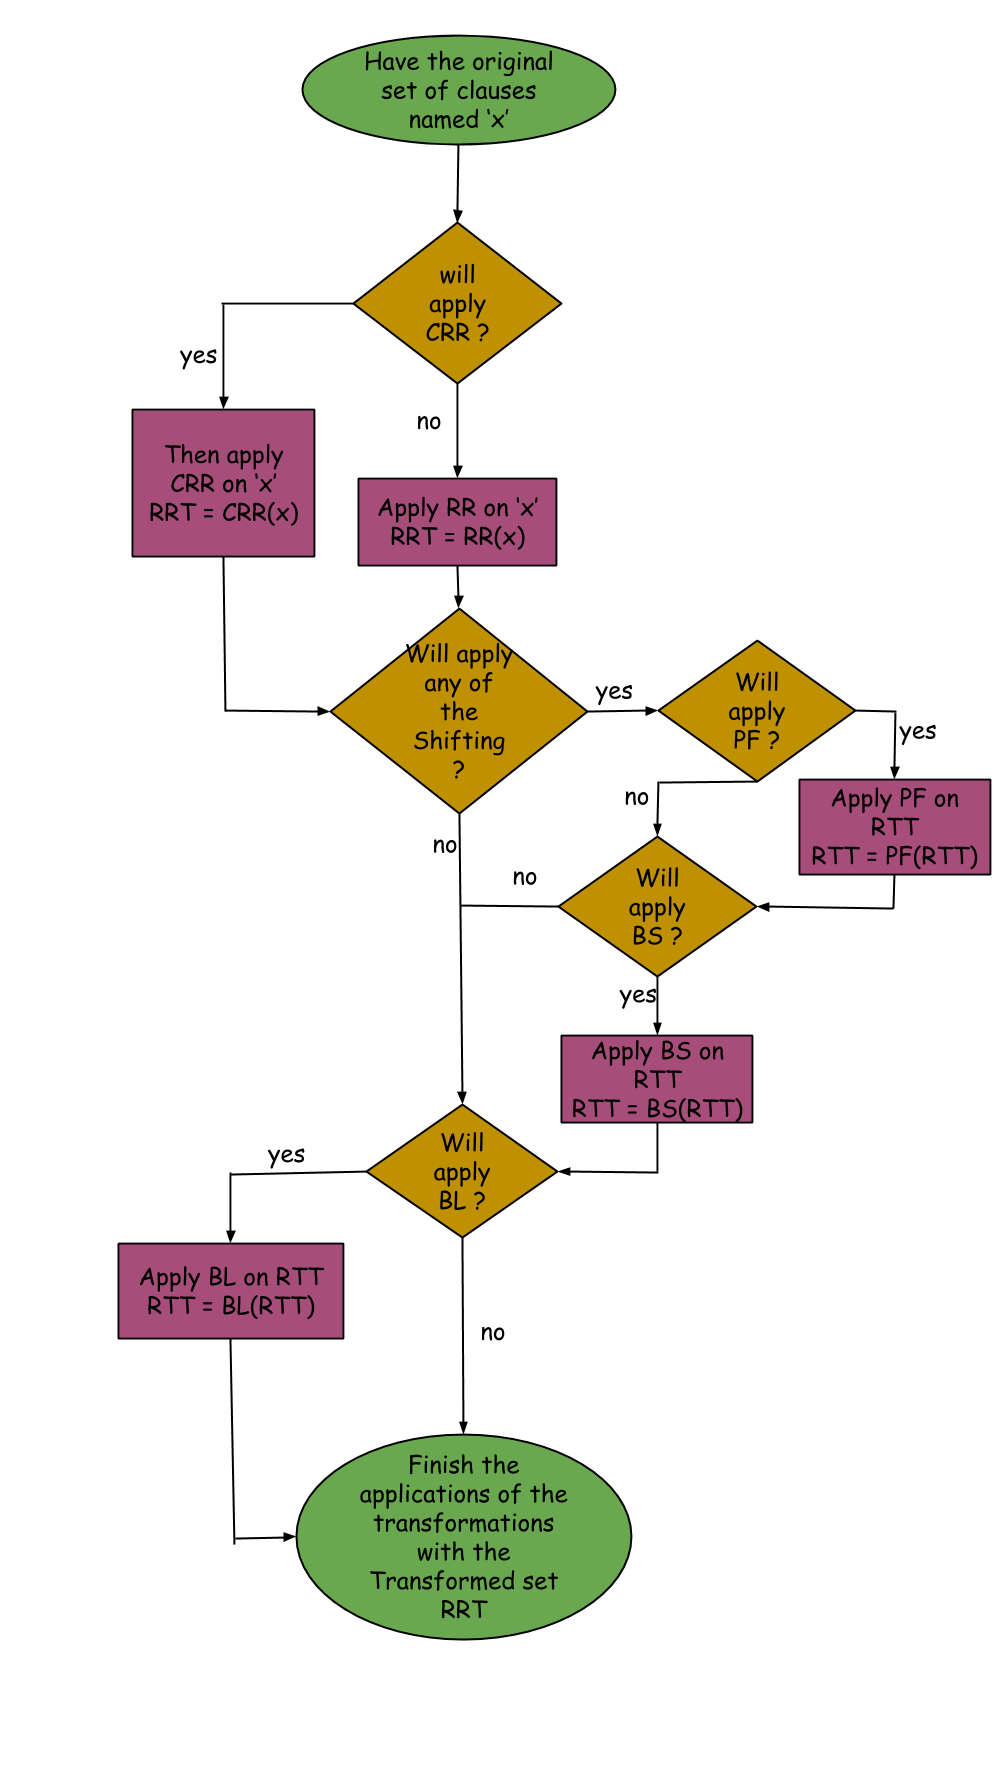
\includegraphics{pictures/Original_transformations_flow.png}}
 			\caption{Flow of the original transformations}\label{fig:original_transformations_flow}
		\end{figure}
	\subsection{Simplified transformations}\label{sub:c3s1s2}

This part is concerned about discussing the simplifications that were added to the original transformations highlighted in \ref{sub:c3s1s1}.
\\
Keeping in mind the definition of \ac{epr} as mentioned here in \ref{sub:c2s1s4}.
\\
So the following were made to each of the procedures:
\\
1- Every step that only deals with proper function symbols is removed since they are not existing in \ac{epr}.
\\
2- Any step or procedure that was introduced because of the existence of problems because of proper function symbols were removed as well. Ex.: pf, sh, and bl.
\\
\\
Therefore the resultant simplified procedures are the following:
\\
For crr:
\\
(0) Initialization. Initially, let crr(M) := M.
\\
(1) Add a constant. Let dom be a “fresh” unary predicate symbol not in ΣP , and let c
be some constant. Extend crr(M) by the clause dom(c) ← . (The constant c can
be “fresh” or belong to Σ f .)
\\
(2) Range-restriction. For each clause H ← B in crr(M), let {x1 , . . . , xk } be the set of
variables occurring in H but not in B . Replace H ← B by the clause
H ← B ∧ dom(x1 ) ∧ · · · ∧ dom(xk ).
\\
\\
For rr:
\\
(0) Initialization. Initially, let rr(M) := M.
\\
(1) Add a constant. Same as Step (1) in the definition of crr.
\\
(2) Domain elements from clause bodies. For each clause H ← B in M and each atom
P(t1 , . . . ,tn ) from B , let P(s1 , . . . , sn ) be the term abstraction of P(t1 , . . . ,tn ) and let α be the corresponding abstraction substitution. Extend rr(M) by the set
{dom(xi )α ← P(s1 , . . . , sn ) | 1 ≤ i ≤ n and xi → ti ∈ α}.
\\
(3) Range-restriction. Same as Step (2) in the definition of crr.
\\
(4) Domain elements from ΣP . For each n-ary P in Σ p , extend rr(M) by the set
{dom(xi ) ← P(x1 , . . . , xn ) | i ≤ i ≤ n}.


  
	

	\section{Code Flow}